\section{Experimental Results\label{sec:results}}

In experiments on the English and Spanish TAC KBC slot-filling tasks, we find that both USchema and LSTM models outperform the CNN across languages, and that the LSTM tends to perform slightly better than USchema as the only model. Ensembling the LSTM and USchema models further increases final F1 scores in all experiments, suggesting that the two different types of model compliment each other well. Indeed, in Section \ref{sec:uschema-lstm} we present quantitative and qualitative analysis of our results which further confirms this hypothesis: In experiments characterizing the behavior of the LSTM and USchema models we find that they perform better on different pattern lengths and are characterized by different precision-recall tradeoffs.

\subsection {English TAC Slot-filling Results}


\begin{table}[t!]
\setlength{\tabcolsep}{4.1pt}
\begin{center}
\begin{tabular}{|lrrr|}
\hline
\bf Model & \bf Recall & \bf Precision & \bf F1 \\
\hline\hline
CNN                 & 31.6 & 36.8 & 34.1 \\
%CNN-parse           & ?	& ? & ? \\
LSTM                & 32.2 & 39.6 & \bf 35.5  \\
USchema             & 29.4 & 42.6 & 34.8 \\
\hline\hline
USchema+LSTM        & 34.4 & 41.9 & 37.7 \\
USchema+LSTM+Es        & 38.1 & 40.2 & \bf 39.2 \\
\hline\hline
USchema+LSTM+AN	& 36.7 & 43.1 & 39.7 \\
USchema+LSTM+Es+AN & 40.2 & 41.2 & \bf 40.7 \\
\citet{roth2014relationfactory} & 35.8 & 45.7 & 40.2 \\
%\hline\hline
%\citet{angeli2014stanford}* & --- & --- & 40.9 \\
%USchema+LSTM+Es+AN * &	43.1 & 41.2	& \bf 42.1 \\

\hline
\end{tabular}
\caption{Precision, recall and F1 on the English TAC 2013 slot-filling task. AN refers to alternative names heuristic and Es refers to the addition of Spanish text at train time. LSTM+USchema ensemble outperforms any single model, including highly-tuned competitive systems of \protect\citet{roth2014relationfactory} and \protect\citet{angeli2014stanford}, despite using no handwritten patterns.  %both use hand written patterns. * = optimal per relation tuning
\label{en-tac-table}}
\end{center}
\end{table}

\begin{table}[t!]
\begin{center}
\begin{tabular}{|lrrr|}
\hline
\bf Model & \bf Recall & \bf Precision & \bf F1 \\
\hline\hline
CNN                 & 28.1 & 29.0 & 28.5 \\
%CNN-parse           & ?	& ? & ? \\
LSTM                & 27.3 & 32.9 & \bf 29.8  \\
USchema             & 24.3 & 35.5 & 28.8 \\
\hline\hline
USchema+LSTM        & 34.1 & 29.3 & 31.5 \\
USchema+LSTM+Es        & 34.4 & 31.0 & \bf 32.6 \\
%USchema+LSTM+AN        & 34.7 & 29.3 & 31.7 \\
%USchema+LSTM+AN+Es        & 33.5 & 32.2 & \bf 32.8 \\
\hline\hline
UT Austin & 25.7 & 42.8 & 32.1 \\
ICTAS\_OKN & 24.3 & 59.0 & 34.4 \\
RPI Blender & 29.4 & 47.8 & 36.4 \\
\citet{angeli2014stanford} & 29.8 & 58.5 & \bf 39.5 \\

\hline
\end{tabular}
\caption{Precision, recall and F1 on the English TAC 2014 slot-filling task. Es refers to the addition of Spanish text at train time. The AN heuristic is ineffective on 2014 adding only 0.2 to F1. We include results for the top 4 performing systems in the official TAC 2014 competition. Our system would rank 4/18 behind systems that use hand-written patterns and active learning despite our system using neither of these additional annotations \protect\citep{SurdeanuMihai2014}.\label{2014-en-tac-table}}
\end{center}
\end{table}

Tables \ref{en-tac-table} and \ref{2014-en-tac-table} present the performance of our models on the 2013 and 2014 English TAC slot-filling tasks. Ensembling the LSTM and USchema models improves F1 by 2.2 points for 2013 and 1.7 points for 2014 over the strongest single model on both evaluations, LSTM. Adding the alternative names (AN) heuristic described in Section \ref{sec:models} increases F1 by an additional 2 points on 2013, resulting in an F1 score that is competitive with the state-of-the-art. We also demonstrate the effect of jointly learning English and Spanish models on English slot-filling performance. Adding Spanish data improves our F1 scores by 1.5 points on 2013 and 1.1 on 2014 over using English alone. This places are system higher than the top performer at the 2013 TAC slot-filling task even though our system uses no hand-written rules.

The state of the art systems on this task all rely on matching handwritten patterns to find additional answers and the top 2014 system uses additional active learning annotation to get higher quality training data. Our models use only automatically generated, indirect supervision; even our AN heuristics (Section \ref{sec:pipeline}) are automatically generated. Our model performs substantially better on 2013 than 2014 for two reasons. First, our RelationFactory\citep{roth2014relationfactory} retrieval pipeline was designed for the 2013 task, but the 2014 task introduced new challenges such as confusable entities. Second, improved training using active learning gave the top 2014 systems a very large boost in performance. No 2013 systems, including ours, use active learning. \todo{do we need more justification for our less good 2014 results?}


%\begin{table}[tb]
%\begin{center}
%\caption{Precision, recall and F1 of English-only models on the English TAC 2012 slot-filling task. \label{2012-en-tac-table}}
%\begin{tabular}{|lrrr|}
%\hline
%\bf Model & \bf Recall & \bf Precision & \bf F1 \\
%\hline\hline
%CNN                 & 28.5 & 26.0 & 27.2 \\
%LSTM                & 26.9 & 27.1 & 27.0  \\
%USchema             & 22.0 & 34.2 & 26.8 \\
%\hline\hline
%USchema+LSTM        & 30.2 & 26.7 & 29.1 \\
%\citet{angeli2014stanford}* & --- & --- & 30.7 \\
%\hline
%\end{tabular}
%\end{center}
%\end{table}


\subsection{USchema vs LSTM \label{sec:uschema-lstm}}

\begin{figure}[t!]
\begin{center}
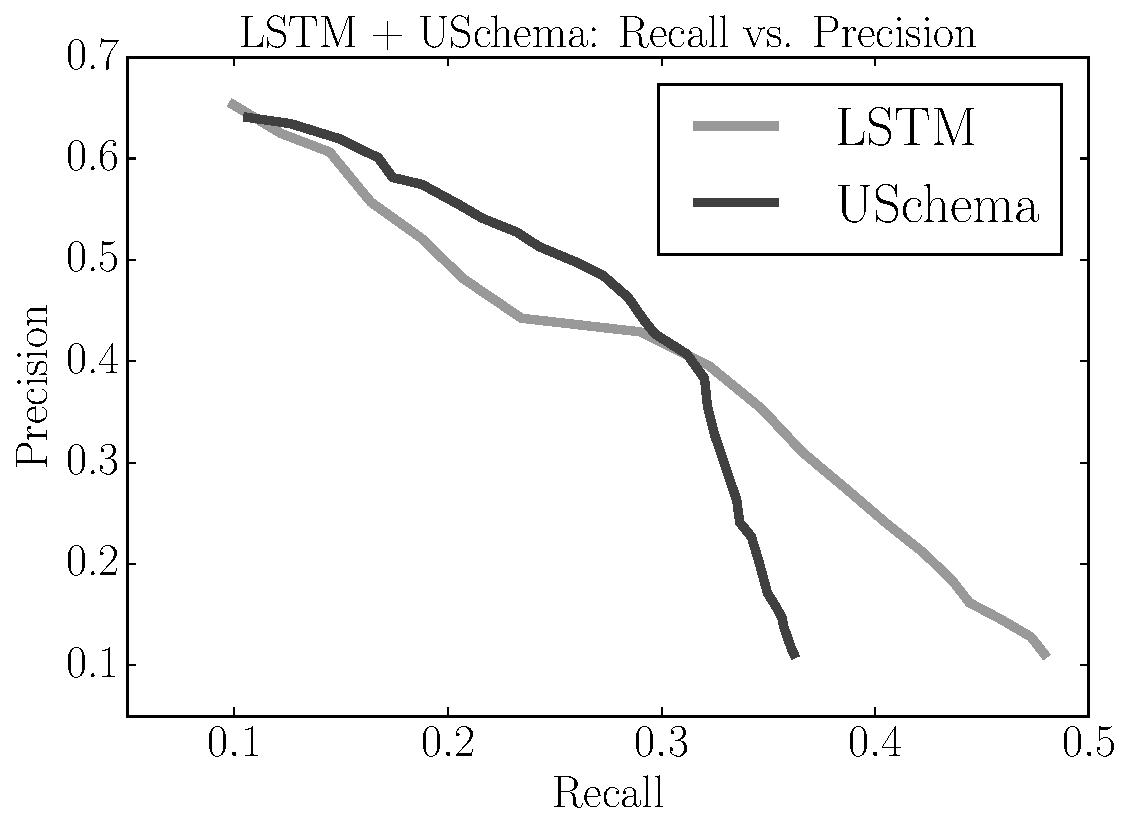
\includegraphics[scale=0.45]{pr-curve}
\caption{Precision-Recall curves for USchema and LSTM on 2013 TAC slot-filling. USchema achieves higher precision values whereas LSTM has higher recall. \label{fig:pr-curve}}
\end{center}
\end{figure}

\begin{figure}[t!]
\begin{center}
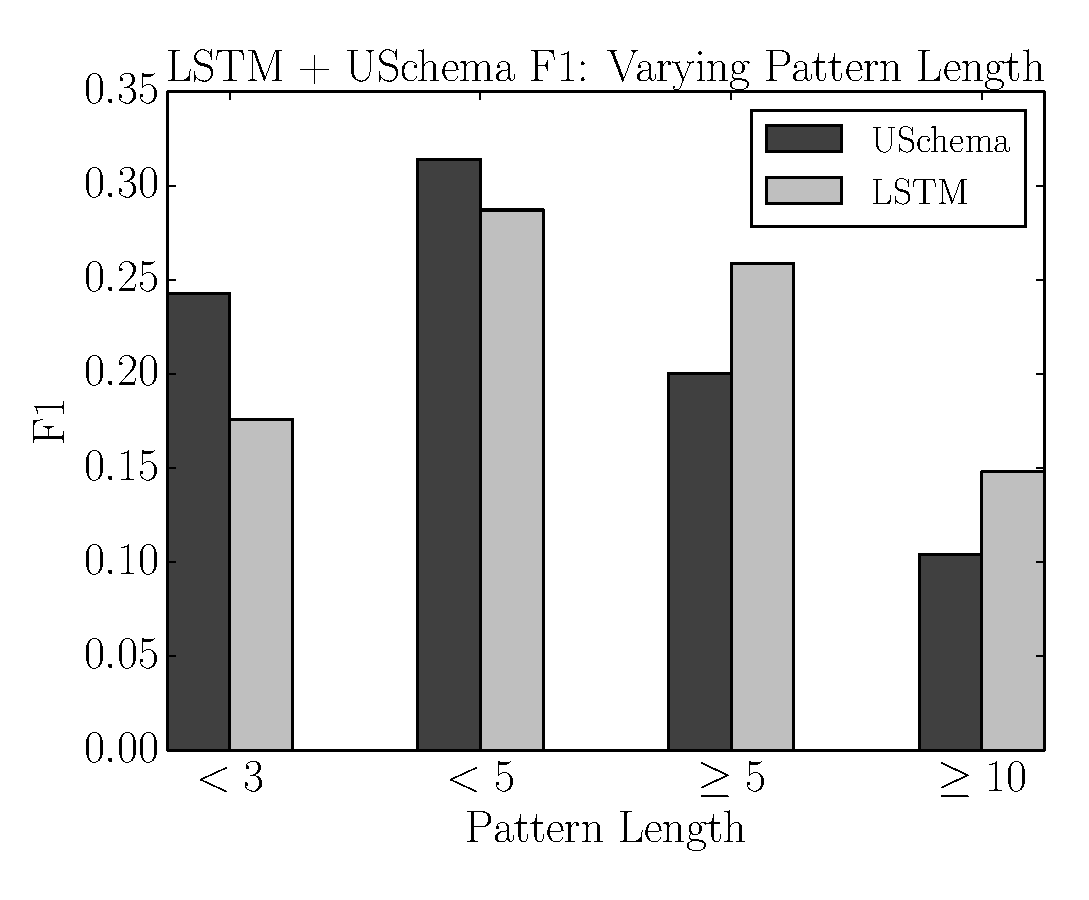
\includegraphics[scale=0.45]{f1-vary-pat-length}
\caption{F1 achieved by USchema vs. LSTM models for varying pattern lengths on 2013 TAC slot-filling. LSTM performs better on longer patterns ($\geq$ 5 tokens) whereas USchema performs better on shorter patterns ($\leq 5$). \label{fig:f1-vary-pats}}
\end{center}
\end{figure}

We further analyze differences between USchema and LSTM in order to better understand why ensembling the models results in the best performing system. Figure \ref{fig:pr-curve} depicts predicion-recall curves for the two models on the 2013 slot-filling task. As observed in earlier results, we see that the LSTM achieves higher recall at the loss of some precision, whereas USchema can make more precise predictions at a lower threshold for recall. In Figure \ref{fig:f1-vary-pats} we observe evidence for these different precision-recall tradeoffs: USchema scores higher in terms of F1 on shorter patterns whereas the LSTM scores higher on longer patterns. As one would expect, USchema successfully matches more shorter patterns on average than the LSTM, making more precise predictions at the cost of being unable to predict on patterns unseen during training. The LSTM can predict using any text between entities observed at test time, gaining recall at the loss of precision. Combining the two models makes the most of their strengths and weaknesses, leading to the highest overall F1.


% error analysis
Qualitative analysis of our English models also suggests that our encoder-based models (LSTM) extract relations based on a wide range of semantically similar patterns that the pattern-matching model (USchema) is unable to score due to a lack of exact string match in the test data. For example, Table \ref{tab:lstm-us-similar-rels} lists three examples of the \emph{per:children} relation that the LSTM finds which USchema does not, as well as three patterns that USchema does find. Though the LSTM patterns are all semantically and syntactically similar, they each contain different specific noun phrases, e.g. \emph{Lori}, \emph{four children}, \emph{toddler daughter}, \emph{Lee and Albert}, etc. Because these specific nouns weren't seen during training, USchema fails to find these patterns whereas the LSTM learns to ignore the specific nouns in favor of the overall pattern, that of a parent-child relationship in an obituary. USchema is limited to finding the relations represented by patterns observed during training, which limits the patterns matched at test-time to short and common patterns; all the USchema patterns matched at test time were similar to those listed in Table \ref{tab:lstm-us-similar-rels}: variants of \emph{'s son, '}.


\begin{table}[h]
\begin{center}
\small
\begin{tabular}{|p{7.6cm}|}
\hline
\multicolumn{1}{|c|}{\textbf{LSTM}} \\ \hline
{\bf McGregor} \emph{is survived by his wife, Lori, and four children, daughters Jordan,} { \bf Taylor} and Landri, and a son, Logan. \\ \hline
In addition to his wife, {\bf Mays} \emph{is survived by a toddler daughter and a son,} {\bf Billy Mays Jr.}, who is in his 20s. \\ \hline
{\bf Anderson} \emph{is survived by his wife Carol, sons Lee and Albert, daughter} {\bf Shirley Englebrecht} and nine grandchildren. \\
\hline\hline
\multicolumn{1}{|c|}{\textbf{USchema}}  \\ \hline
{\bf Dio} \emph{'s son,} {\bf Dan Padavona}, cautioned the memorial crowd to be screened regularly by a doctor and take care of themselves, something he said his father did not do. \\ \hline
But {\bf Marshall} \emph{'s son,} {\bf Philip}, told a different story.  \\ \hline
``I'd rather have Sully doing this than some stranger, or some hotshot trying to
be the next Billy Mays,'' said the guy who actually is the next {\bf Billy Mays}\emph{, his son} {\bf Billy Mays III}. \\
\hline
\end{tabular}
\caption{Examples of the \emph{per:children} relation discovered by the LSTM and Universal Schema. Entities are bold and patterns italicized. The LSTM models a richer set of patterns \label{tab:lstm-us-similar-rels}}
\end{center}
\end{table}




\subsection{Spanish TAC Slot-filling Results \label{sec:qual-anal}}

\begin{table}
\begin{center}
\begin{tabular}{|lrr|}
\hline
\bf Model & \bf Es+En & \bf Es+En+dict  \\
\hline\hline
CNN 		                    & 11.4     & 13.8	\\
LSTM 	                        & 10.7     & 15.2   \\
USchema                         & 16.3     & --- \\
\hline
USchema+LSTM                    & 17.3     & \bf 20.0 \\
\hline
\end{tabular}
\caption{Zero-annotation transfer learning F1 scores on 2012 Spanish TAC KBP slot-filling task. Adding a translation dictionary improves all encoder-based models. Ensembling LSTM and USchema models performs the best. \label{es-tac-table}}
\end{center}
\end{table}

Table \ref{es-tac-table} presents 2012 Spanish TAC slot-filling results for our multilingual relation extractors trained using zero-annotation transfer learning. For both the CNN and LSTM, tying word embeddings between the two languages results in substantial improvements. We see that ensembling the non-dictionary LSTM with USchema gives a slight boost over USchema alone, but ensembling the dictionary-tied LSTM with USchema provides a significant increase of nearly 4 F1 points over the highest-scoring single model, USchema. Clearly, grounding the Spanish data using a translation dictionary provides much better Spanish word representations. These improvements are complementary to the baseline USchema model, and yield impressive results when ensembled.

% cross lingual relations
Qualitative analysis of our multilingual models further suggests that they successfully embed semantically similar relations across languages using tied entity pairs and translation dictionary as grounding. Table \ref{tab:cross-lingual-relations} lists three top nearest neighbors in English for several Spanish patterns from the text. In each case, the English patterns capture the relation represented in the Spanish text. 

\newcommand{\tablespace}{\end{tabular}
\newline
\newline
%\hspace*{-21pt}
\begin{tabular}{|p{7.6cm}|}
}
\begin{table}[h]
\begin{center}
\small
%\hspace*{-21pt}
\begin{tabular}{|p{7.6cm}|}
\hline
 \bf y cuatro de sus familias, incluidos su esposa, \endgraf \hspace{5pt}Wu Shu-chen, su hijo, \\
\it{ and four of his family members, including his wife, \endgraf \hspace{5pt}Wu Shu-chen, his son, } \\
\hline
 and his son  \\
 is survived by his wife, Sybil MacKenzie and a son,  \\
 gave birth to a baby last week -- son  \\
\hline
\tablespace
\hline
 \bf (Puff Daddy, cuyos verdaderos nombre sea  \\
\it{ (Puff Daddy, whose real name is } \\
\hline%\hline
 (usually credited as {\it E1} \\
 (also known as Gero \#\#, real name  \\
 and (after changing his name to  \\
\hline
\tablespace
%\hline
%, Tian Tian, de \#\# a\~{n}os de edad, y su madre \\
%\it{, Tian Tian, \#\# years old, and his mother } \\
%\hline%\hline
% Gyllenhaal's parents -- screenwriter Naomi Foner and director  \\
% Brando's mother, actress Anna Kashfi, divorced  \\
% Cash, his mom was  \\
%\hline
%\tablespace
\hline
 \bf lleg\'{o} a la alfombra roja en compa\~{n}\'{i}a de su esposa, la \endgraf \hspace{5pt} actriz  Suzy Amis, casi una hora antes que su ex esposa, \\
\it{ arrived on the red carpet with his wife, \endgraf \hspace{5pt} actress  Suzy Amis, nearly an hour before his ex-wife , } \\
\hline%\hline
, who may or may not be having twins with husband  \\
, aged twenty, Kirk married \\
 went to elaborate lengths to keep his wedding to former \endgraf \hspace{5pt}supermodel \\
\hline
%\tablespace
%\hline
%\bf{{\it E1} , una firmes of estudios económicos lleven sede in {\it E2}}\\
%\it{{\it E1} an economic studies firm with headquarters in {\it E2}} \\
%\hline\hline
%{\it E2} offices of BP and {\it E1} \\
%{\it E2} , the Paris - based {\it E1} \\
%{\it E2} province , is the headquarters of {\it E1} \\
%\hline
\end{tabular}
\caption{Top English patterns for a Spanish query pattern encoded using the dictionary LSTM: For each Spanish query (English translation in italics), a list of English nearest neighbors. \label{tab:cross-lingual-relations}}
\end{center}
\end{table}


In addition to embedding semantically similar phrases from English and Spanish to have high similarity, our models also learn high-quality multilingual word embeddings. In Table \ref{joint-word} we compare Spanish nearest neighbors of English query words learned by the LSTM with dictionary ties versus the LSTM with no ties, using no unsupervised pre-training for the embeddings. Both approaches jointly embed Spanish and English word types, using shared entity embeddings, but the dictionary-tied model learns qualitatively better multilingual embeddings. See Section \ref{sec:more-qual-anal} for additional qualititave results.


\begin{table}[h]
\setlength{\tabcolsep}{3pt}
\small
\begin{center}
%\begin{minipage}[b]{0.45\linewidth}
%\hspace*{-17pt}
\begin{tabular}{|ll|}
\hline
\multicolumn{2}{|c|}{ \bf CEO}\\
\multicolumn{1}{|c}{Dictionary} & \multicolumn{1}{c|} {No Ties} \\ \hline 
jefe (chief)    & CEO \\ 
CEO & director (principle) \\
ejecutivo (executive)   &  directora (director) \\
cofundador (cofounder)  & firma (firm) \\
president (chairman) & magnate (tycoon)\\
\hline
%
\multicolumn{2}{|c|}{\bf headquartered}\\
\multicolumn{1}{|c}{Dictionary} & \multicolumn{1}{c|} {No Ties} \\ \hline
sede (headquarters) & Geol\'{o}gico (Geological) \\
situado (located) & Treki (Treki) \\
selectivo (selective) & Geof\'{i}sico(geophysical) \\
profesional (vocational) & Normand\'{i}a (Normandy)\\
bas\'{a}ndose (based) & emplea (uses)\\
\hline
%\end{tabular}
%\end{minipage}
%\hspace{-12.5pt}
%\begin{minipage}[b]{0.45\linewidth}
%\begin{tabular}{|ll|}
%\hline
\multicolumn{2}{|c|}{\bf hubby}\\
\multicolumn{1}{|c}{Dictionary} & \multicolumn{1}{c|} {No Ties} \\ \hline 
matrimonio (marriage)  & esposa (wife) \\ 
casada (married) & esposo (husband) \\
esposa (wife) &  casada(married) \\
cas\'{o} (married) & embarazada (pregnant)  \\
embarazada (pregnant) & embarazo (pregnancy) \\
\hline

%
\multicolumn{2}{|c|}{\bf alias}\\
\multicolumn{1}{|c}{Dictionary} & \multicolumn{1}{c|} {No Ties} \\ \hline
simplificado (simplified) & Weaver (Weaver)\\ 
sabido (known) & interrogaci\'{o}n (question) \\
seud\'{o}nimo (pseudonym)  &  alias \\
privatizaci\'{o}n (privatisation)  & reelecto (reelected) \\
nombre (name)  & conocido (known)\\
\hline
\end{tabular}
\caption{Example English query words (not in translation dictionary) in bold with their top nearest neighbors by cosine similarity listed for the dictionary and no ties LSTM variants. Dictionary-tied nearest neighbors are consistently more relevant to the query word than untied. \label{joint-word}}
%\end{minipage}
\end{center}
\end{table}




